Structural assessment of the inflatable configuration has been performed by an estimation of internal forces. This is an essential step in the design of an inflatable aeroshell, since a force estimation:
\begin{itemize}
\item Is required to estimate the inflation pressure to maintain its structural integrity and aerodynamic shape under peak aerodynamic loading
\item Allows to identify whether loads allow for concept structural design within state-of-the-art material capabilities
\item Yields the loads at the structural interface between the inflatable aeroshell and the rigid centerbody
\item Gives an impression of the effect of changing design parameters on concept structural performance
\end{itemize}
Forces are estimated for an inflatable structure that is aerodynamically loaded, as follows from vehicle trajectory analysis in Chapter \ref{ch:XXX}, in its deployed condition. An interface with the aerodynamic analysis, performed in Chapter \ref{ch:XXX}, yields the optimized aeroshell shape as a baseline for the structural model used.

\subsubsection{Approach outline}
To meet the purposes of structural assessment of the inflatable configuration, force estimation is performed by a two-dimensional truss analysis on a simplified geometry. This geometry relies on the aerodynamic aeroshell shape, optimized in Chapter \ref{ch:XXX}, to define its outer shape. This shape is effected by a number of toroids \gls{sym:N}, held together by radial straps, running along the surface of the inflatable. 

Adjoining toroids are connected at three locations: by a radial strap along the forward side of the aeroshell (impinged by the flow), a radial strap running along the aft side of the aeroshell and at their direct contact surface. In reality, as in the stacked toroid configuration used for NASAs \gls{irve} \cite{Lindell2006}, the contact surface of adjoining toroids is a straight wall, while top and bottom surfaces are of circular shape. This shape is the result of the internally applied pressure: equal but oppositely directed pressures effect a straight interface between toroids and toroids adapt to the unbalanced pressure in top and bottom surfaces through energy minimization by taking a circular shape.

Simplification was performed to realize a structurally determinate problem results by modelling toroids as diamonds. The orientation of the diamonds is defined by the half-cone angle \gls{sym:theta}, allowed to vary over its radius and circumference per toroid, and their shape by a fixed width \gls{sym:w} and varying height \gls{sym:h}, to allow for a tapered structure. Nodes are designated as the corners of each diamond and connecting members have been numbered. The numbering convention and dimensions are illustrated in Figure \ref{fig:TC}. 

\begin{figure}[h]
	\centering
	\begin{subfigure}[b]{0.49\textwidth}
	\centering
	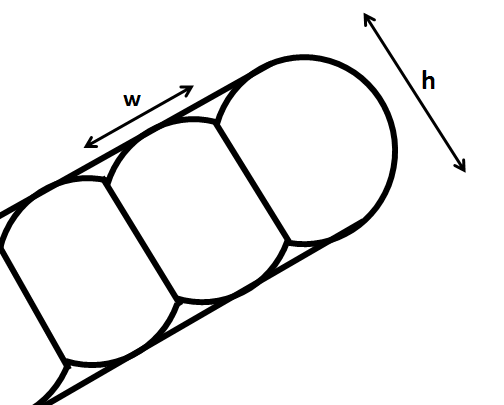
\includegraphics[width=1.0\textwidth]{./Figure/Structure/ToroidConfig.png}
	\caption{Actual toroid layout} 
	\label{fig:TC1}
	\end{subfigure}
	\begin{subfigure}[b]{0.49\textwidth}
	\centering
	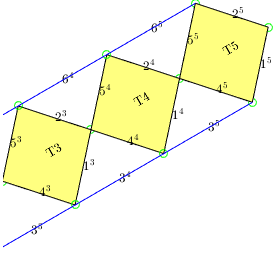
\includegraphics[width=1.0\textwidth]{./Figure/Structure/ToroidConfig2.png}
	\caption{Simplified truss model} 
	\label{fig:TC2}
	\end{subfigure}
	\caption{Comparison between the actual and simplified inflatable model}
	\label{fig:TC}
\end{figure}

Force estimation is performed in a two-dimensional plane representing a cross-sectional slice, of an infinitesimal angle, of the sphere cone. Each toroid is loaded externally by an aerodynamic force applied perpendicular to its width \gls{sym:w} at its forward node (placed directly in the flow). The aerodynamic force is the resultant of the limit aerodynamic pressure $\gls{sym:q}_{limit}$, assumed constant for each toroid, multiplied by toroid width \gls{sym:w} to represent its working area. The limit aerodynamic pressure is determined from the peak dynamic pressure by multiplying with a \acrfull{fos}, thereby taking into account a contingency for structural design. For composite structures, NASA dictates a \gls{fos} of 1.5 for uniform material and 2.0 for a discontinuity area \cite{Technical2014}. As the inflatable comprises a large amount of component interaction and discontinuity, the ultimate load is calculated as twice the limit aerodynamic pressure that follows from the trajectory analysis in Chapter \ref{ch:XXX}.

In addition to the aerodynamic pressure acting on the inflatable forward surface, movables (e.g. flaps) at the edge of the aeroshell are taken into account, where present, as a point load, of prescribed magnitude by control considerations following from Chapter \ref{ch:XXX}, directed perpendicular to the flap deployed surface area.

As input forces are in Newtons per meter, being the product of a pressure over a length, forces should technically be designated as forces per unit length or running loads. Hereafter, all references to forces in this section are in fact references to running loads. To calculate forces from running loads, these should be multiplied with the circumference over which they act.

On the basis of these external forces, estimation is performed by a truss analysis. By requiring force equilibrium in two orthogonal directions within the plane, internal forces in each of the members 1 to 6 for the \gls{sym:N} toroids are determined. This system of equations is solved from the free end (outboard) to the pinned end (inboard) where the inflatable is connected to the centerbody. At this location, reaction forces in two orthogonal directions are determined at the two attachment points, forward and aft.

The decreasing circumference over which forces act going from outboard to inboard in each two-dimensional slice, inherent to the sphere cone design, effects a proportional increase in running loads. This increase is proportional to the decrease in diameter, via the circumference, and thereby member forces are scaled by the ratio of radial distances, with respect to the centerbody longitudinal axis, of the nodes they connect.

After this first iteration, internal pressure is to be taken into account. It is calculated as the pressure that brings all members into tension, based on the following reasoning. In case members are in compression, buckling will reduce the load-carrying capability of the structure. For the inflatable structure, buckling occurs at low loads due to its flexible and foldable nature. Therefore, the flexible material of the inflatable is not to be loaded into compression and required to be in tension. The latter is effected by the inflation pressure, which is estimated as follows. The first iteration, without inflation pressure, yields internal forces in all members. The requirement for internal pressure is that its induced force $\gls{sym:G}_{infl}$ (or running load), calculated via Equation \ref{eq:pressureforce} \cite{XXX}
\begin{equation}
G_{infl} = \frac{p_{infl} w}{2}
\label{eq:pressureforce}
\end{equation}
brings all members into tension. Dimension \gls{sym:w} is used for all toroids, as it is smaller than \gls{sym:h} and therefore a more conservative estimate for the inflation pressure results. For the outer toroid, the inflation pressure is predominantly carried by the radial straps and this leads to the first requirement that the radial straps are loaded in tension. For all other toroids, the inflation pressure internally balances itself and is thereby not carried through the structure (and radial straps), since cells are symmetric and adjoining cells have the same inflation pressure. This leads to the second requirement that all toroid walls are in tension. Based hereupon, the second iteration proceeds by setting the pressure equal to the value that satisfies the second requirement. Subsequent iterations continue to increase the inflation pressure until the first requirement is met. 

The inputs of the structural model are:
\begin{itemize}
\item Toroid inclination in terms of local half-cone angle \gls{sym:theta}
\item Number of toroids \gls{sym:N}
\item Toroid dimensions in terms of width \gls{sym:w} and height \gls{sym:h}
\item Aerodynamic loading in terms of dynamic pressure \gls{sym:q}
\item Centerbody diameter \gls{sym:Di}
\item Deployed diameter \gls{sym:Do}
\end{itemize}
Based on these inputs, outputs of the structural model are:
\begin{itemize}
\item Internal forces (running loads) in each of the members of all toroids
\item Reaction forces at the connection to the centerbody of forward and aft radial strap respectively
\item Inflation pressure \gls{sym:pinfl} required to bring all members into tension
\end{itemize}

\subsubsection{Assumptions}
This approach relies on the following assumptions:

\begin{itemize}
\item Small deformations. In reality deformations can be significant changing the orientation and magnitude of forces in the structure.
\item No three dimensional effects. Neglecting the three dimensional effects impacts the stiffness, and the ability to carry lateral loads of the structure. The former is not considered as also mentioned above. The latter causes a over estimation of the horizontal loads (as per figure \ref{fig:TC}).  
\item Constant dynamic pressure. A constant dynamic pressure is not in line with the actual loading, errors are however small and irrelevant as compared the other assumptions.
\item The loading is applied discrete at the outer nodes. The effects of a continuous distribution are neglected since they do not fit within the truss model. This assumptions neglects a bending load within the forward radial strap.
\item Structural mass is neglected. Neglecting the structural mass causes a small error within the computed loads. These errors are however insignificant as compared to the other assumptions.
\end{itemize} 

The effects of these assumptions is in total quite significant. The method relies heavily on the first and second assumption. Considering the foldable nature of the structure, stiffness is limited and actual deformations may become significant. This assumptions is partly taken into account by requiring a inflation pressure which prevents any compressive loading. Still tough further stiffness consideration are not taken into account. Based on the significance of these assumptions actual stress distributions can not be considered. However the applied model is reliable for a more general analysis of the structure and the loads.

\subsubsection{Verification and Validation}

Verification is performed on the basis of simplified load cases. Significant errors were not observed and remained below 3\% for various geometries and halve cone angels with a minimum of 5 tori. The small verification errors followed from the discrete application of the dynamic pressure. Taking the discrete application into account as well the errors disappear.

Validation is performed for the inner root section of the inflatable on the basis of the results presented by Lindell et al. \cite{Lindell2006}. Lindell presents results for the root section of the first \gls{irve} design by means of \gls{fem} analysis. The comparative errors between both methods remain below XX\%. Table \ref{tab:struc_val} presents the results of this validation effort presenting moreover the results of closed form equations valid for solely the root section of the inflatable.

TABLE

It is important to consider that actual local loading may be significantly higher and should be properly accounted for in  possible further detailed design phases. For now this accounted for by the use of contingency factors.
\subsubsection{Results}



